\section{Introduction}
\label{sec:Introduction}

The objective of this laboratoty is to study the behaviour of the circuit using nodal method and mesh method.The curcuit contains both dependent and independent current and voltage source, $I_b$,$I_d$,$V_c$ and $V_a$ respectively.The circuit also has resistors with known resistance.The circuit can be seen in figure~\ref{fig:rc} .



In Section~\ref{sec:analysis}, a theoretical analysis of the circuit is
presented. In Section~\ref{sec:simulation}, the circuit is analysed by
simulation, and the results are compared to the theoretical results obtained in
Section~\ref{sec:analysis}. The conclusions of this study are outlined in
Section~\ref{sec:conclusion}.

\begin{figure}[h] \centering
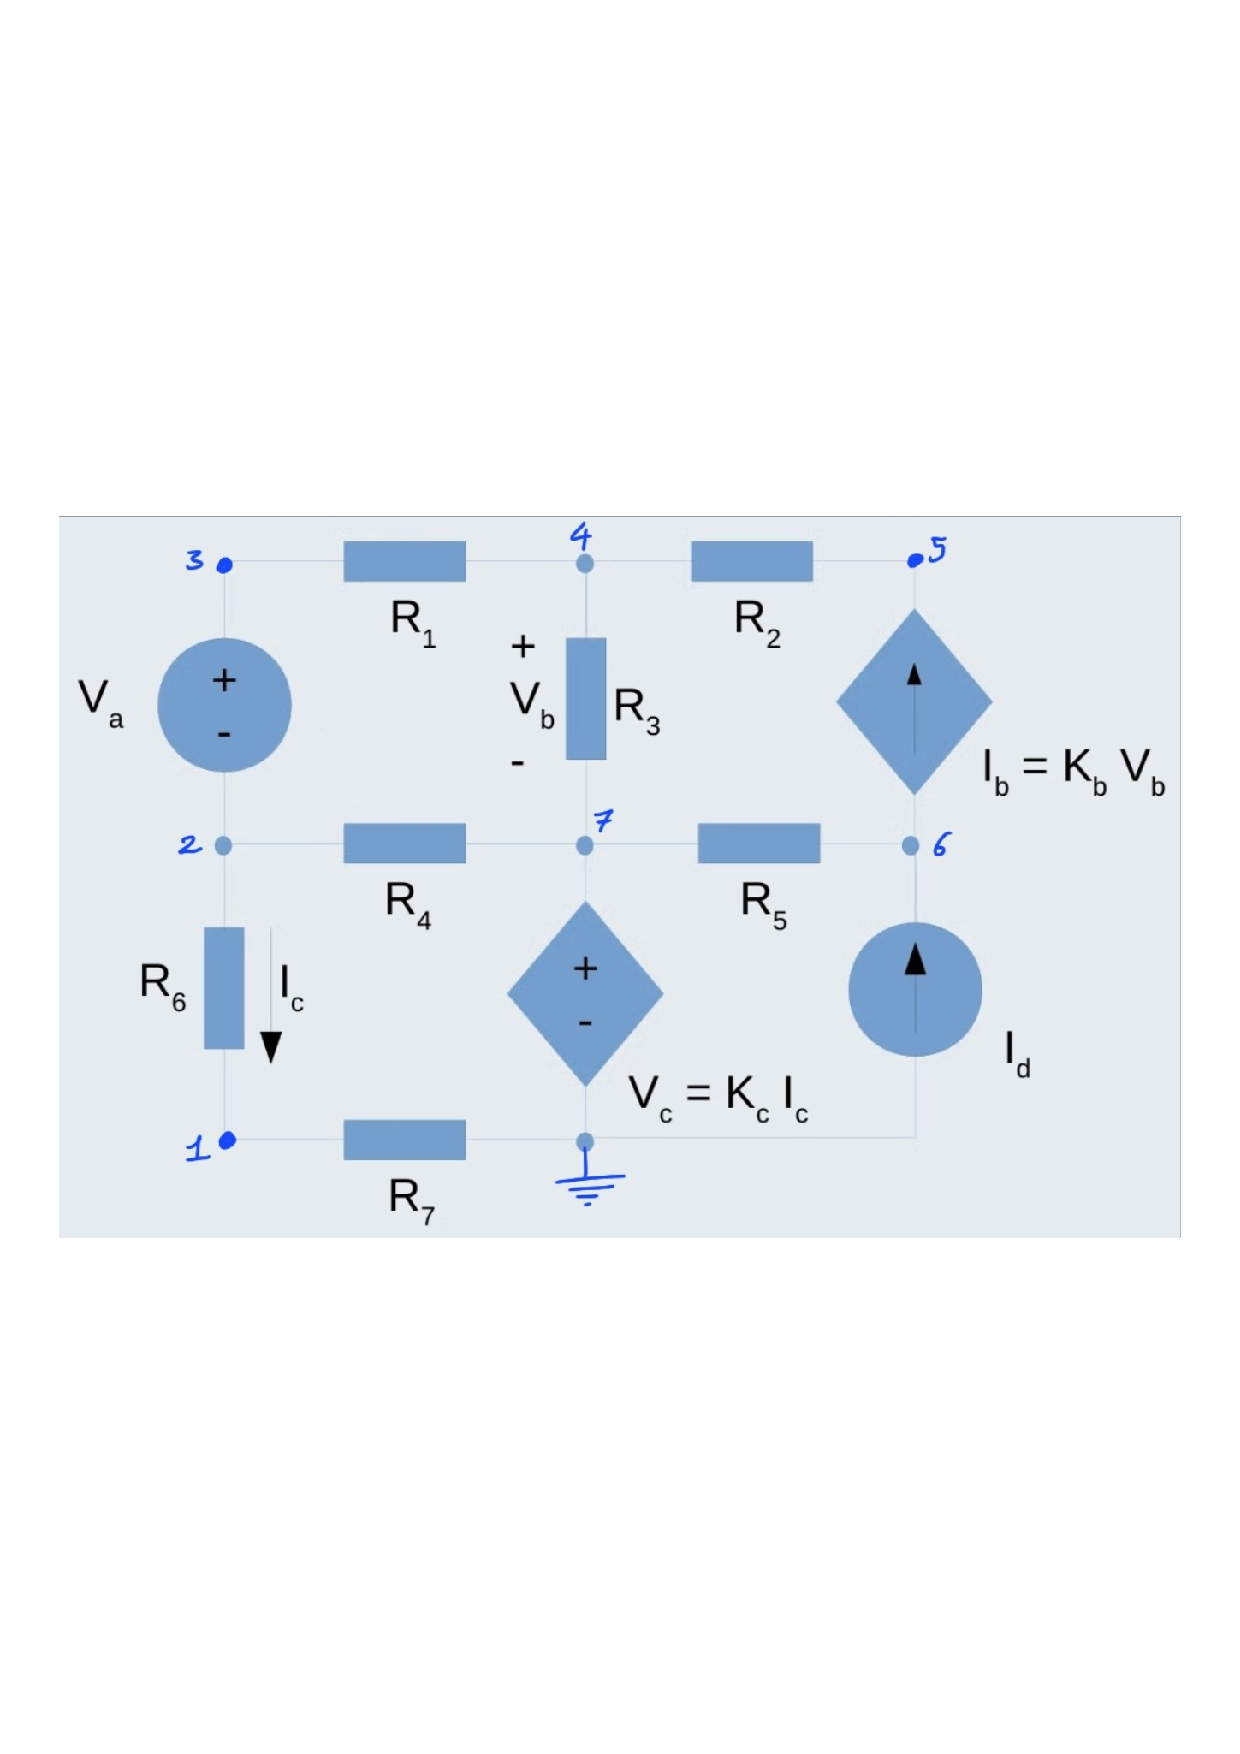
\includegraphics[width=0.7\linewidth]{rc}
\caption{Dependent and Independent sources circuit.}
\label{fig:rc}
\end{figure}

